
\documentclass[a4paper,UKenglish,cleveref, autoref, thm-restate]{lipics-v2021}
%This is a template for producing LIPIcs articles. 
%See lipics-v2021-authors-guidelines.pdf for further information.
%for A4 paper format use option "a4paper", for US-letter use option "letterpaper"
%for british hyphenation rules use option "UKenglish", for american hyphenation rules use option "USenglish"
%for section-numbered lemmas etc., use "numberwithinsect"
%for enabling cleveref support, use "cleveref"
%for enabling autoref support, use "autoref"
%for anonymousing the authors (e.g. for double-blind review), add "anonymous"
%for enabling thm-restate support, use "thm-restate"
%for enabling a two-column layout for the author/affilation part (only applicable for > 6 authors), use "authorcolumns"
%for producing a PDF according the PDF/A standard, add "pdfa"

% \pdfoutput=1 %uncomment to ensure pdflatex processing (mandatatory e.g. to submit to arXiv)
\hideLIPIcs  %uncomment to remove references to LIPIcs series (logo, DOI, ...), e.g. when preparing a pre-final version to be uploaded to arXiv or another public repository
\nolinenumbers

\usepackage{pgfplots}
\pgfplotsset{compat=1.18}
\usepgfplotslibrary{statistics, units, groupplots}

\usepackage{subcaption}

\pgfplotsset{
    only if/.style args={entry of #1 is #2}{
        /pgfplots/boxplot/data filter/.code={
            \edef\tempa{\thisrow{#1}}
            \edef\tempb{#2}
            \ifx\tempa\tempb
            \else
                \def\pgfmathresult{}
            \fi
        }
    }
} 

\usepackage{tikz}
\usetikzlibrary[fadings]

\def\code#1{\texttt{#1}}
\newcommand\prevsum[0]{\ensuremath{\overset{\leftarrow}{\Sigma}_1}}

%\graphicspath{{./graphics/}}%helpful if your graphic files are in another directory

\bibliographystyle{plainurl}% the mandatory bibstyle

\title{Advanced Data Structures - Succinct Bit Vector}

%\titlerunning{Dummy short title} %TODO optional, please use if title is longer than one line

\author{Paul Hegenberg}{Karlsruher Institut für Technologie, Germany \and \url{https://github.com/paulheg/kit_advanced_data_structures}}{urlgh@student.kit.edu}{}{}%TODO mandatory, please use full name; only 1 author per \author macro; first two parameters are mandatory, other parameters can be empty. Please provide at least the name of the affiliation and the country. The full address is optional. Use additional curly braces to indicate the correct name splitting when the last name consists of multiple name parts.

\authorrunning{P. Open Access and P. Public} %TODO mandatory. First: Use abbreviated first/middle names. Second (only in severe cases): Use first author plus 'et al.'

\Copyright{Paul Open Access} %TODO mandatory, please use full first names. LIPIcs license is "CC-BY";  http://creativecommons.org/licenses/by/3.0/

\ccsdesc[100]{Theory of computation~Data structures design and analysis} %TODO mandatory: Please choose ACM 2012 classifications from https://dl.acm.org/ccs/ccs_flat.cfm 

\keywords{Bit Vectors} %TODO mandatory; please add comma-separated list of keywords

% \category{} %optional, e.g. invited paper

% \relatedversion{} %optional, e.g. full version hosted on arXiv, HAL, or other respository/website
%\relatedversiondetails[linktext={opt. text shown instead of the URL}, cite=DBLP:books/mk/GrayR93]{Classification (e.g. Full Version, Extended Version, Previous Version}{URL to related version} %linktext and cite are optional

%\supplement{}%optional, e.g. related research data, source code, ... hosted on a repository like zenodo, figshare, GitHub, ...
%\supplementdetails[linktext={opt. text shown instead of the URL}, cite=DBLP:books/mk/GrayR93, subcategory={Description, Subcategory}, swhid={Software Heritage Identifier}]{General Classification (e.g. Software, Dataset, Model, ...)}{URL to related version} %linktext, cite, and subcategory are optional

%\funding{(Optional) general funding statement \dots}%optional, to capture a funding statement, which applies to all authors. Please enter author specific funding statements as fifth argument of the \author macro.

% \acknowledgements{I want to thank \dots}%optional

%\nolinenumbers %uncomment to disable line numbering



%Editor-only macros:: begin (do not touch as author)%%%%%%%%%%%%%%%%%%%%%%%%%%%%%%%%%%
\EventEditors{John Q. Open and Joan R. Access}
\EventNoEds{2}
\EventLongTitle{42nd Conference on Very Important Topics (CVIT 2016)}
\EventShortTitle{CVIT 2016}
\EventAcronym{CVIT}
\EventYear{2016}
\EventDate{December 24--27, 2016}
\EventLocation{Little Whinging, United Kingdom}
\EventLogo{}
\SeriesVolume{42}
\ArticleNo{23}
%%%%%%%%%%%%%%%%%%%%%%%%%%%%%%%%%%%%%%%%%%%%%%%%%%%%%%

\begin{document}

\maketitle

\begin{abstract}
We introduce an interleaved data structure optimized for CPU cache efficiency to implement \code{rank},
\code{select}, and \code{access} operations. This structure stores vector data and metadata within a
512-bit cache line, using 64-bit blocks. Metadata, as an incremental sum of set bits, supports fast 
rank and select operations with a 12.5\% memory overhead.
The \code{rank} operation achieves constant execution time, by using incremental sums and pop counts.
The \code{select} operation locates the nth bit occurrence via binary search on metadata and linear search,
aided by a byte-level lookup table.
Performance evaluation confirms that pre-computation scales linearly with vector size and \code{select}
execution scales logarithmic, with variations in speed depending on CPU architecture.
\end{abstract}

\section{Algorithm}
In the following section we will present a data structure
that implements \code{rank}, \code{select} and \code{access} operations.
The data structure aims to use the CPU cache as efficiently as possible, by interleaving both
vector information and metadata to fit in the same cache line of 512 bit.
Our bit vector implementation consists of \code{uint64} blocks, of which we can fit 8 inside one cache line
$L_i = (\prevsum, \vec{v}_0, \dots, \vec{v}_6)$.
To speed up the computation of rank and select we need metadata, which we store in the first
64 bits of the line.
This data structure is depicted in Figure~\ref{fig:interleaved}. 
This leaves us with a memory overhead of $12.5\%$. The used metadata $\prevsum$ is an incremental sum of previous bits
set to one. For an efficient build time of the data structure we make use of the pop count $c(\vec{v})$
instruction, which counts the number of 1 bits in a subvector $\vec{v}$, in our case an \code{uint64} number.

\begin{figure}[htbp]
    \centering
    \tikzfading[name=fade right,
            left color=transparent!0,
            right color=transparent!100]
        \tikzfading[name=fade left,
            left color=transparent!100,
            right color=transparent!0]
    \begin{tikzpicture}
        
        \draw[draw opacity=.4,text opacity=.4,path fading=fade left,densely dotted] (-3,0) rectangle node {$\vec{v}_6$} ++(2,1)
            ++ (0,-.5) -- ++(1,0);

        \draw (0,1) rectangle node {$\prevsum$} (2,0) 
            ++ (0,0) rectangle node {$\vec{v}_0$} ++(2,1)
            ++ (0,-.5) -- node[label={\dots}] {} ++(2,0)
            ++ (0,-.5) rectangle node {$\vec{v}_6$} ++(2,1);
        
        \draw[|-|] (0,-.3) -- node[label=below:{Vector Line (512 bit)}] {} ++(8,0);
        \draw[|-|] (0,1.3) -- node[label=above:{64 bit}] {} ++(2,0);

        \draw[draw opacity=.4,text opacity=.4,path fading=fade right,densely dotted] (8,.5) -- ++(1,0) 
            ++(0,-.5) rectangle node {$\prevsum$} ++(2,1);            

    \end{tikzpicture}
    \caption{Interleaved Data Structure}
    \label{fig:interleaved}    
\end{figure}

\subsection{Rank}
The \code{rank} operation is defined as $\text{rank}(\alpha, p) \mapsto n$, where $\alpha \in \{0,1\}$
and $p,n \in \mathbb{N}_0$. Where $n$ is the number of $\alpha$ valued bits set before position $p$.
To calculate $n$ for a given $\alpha, p$ we first have to find the vector line $L_i$ where the
previous sum $\prevsum$ is stored, by calculating $i=\frac{p}{64 \cdot 7}$.
Using $j = \frac{p}{64} \mod 7$ we then know how many subvectors $\vec{v}$ we need to add to $\prevsum$.
Then we can use bit masks and the pop count operation to count the missing 1 bits.
$$
    n' = \prevsum + \sum_{s=0}^{j-1}c(\vec{v}_s) + c(\text{masked}_{m}(\vec{v}_j))\\
$$
Where $m = p \mod 64$, With $\alpha = 1: n = n'$ for $\alpha = 0: n = p - n'$.
Considering the runtime, we need to execute 7 pop count operations at most, since $0 \leq j \leq 6$.
Resulting in a constant execution time.
Since everything fits into one cache line we don't need to load additional information from memory,
which should improve performance.

\subsection{Select}
The \code{select} operation is defined as $\text{select}(\alpha, n) \mapsto p$, where $n \in \mathbb{N}$ and $p$ is the position
of the $n$th $\alpha$ valued bit. With the interleaved data structure we use the incremental sum
to find the vector line with the biggest prev. sum $\prevsum < n$ using a binary search.
The following subvectors $\vec{v}_i$ will therefore contain the $n$th $\alpha$ bit.
To find the position we conduct a linear search utilizing pop count, selecting the first
$\vec{v}_i$ where $c(\vec{v}_i) \geq n$. Next we divide $\vec{v}_i$ into byte sized blocks to apply 
the same linear search to find the byte containing the $n$th bit.
To get the position inside the byte we created a lookup table, which is described further in Section~\ref{p:select_lookup}.

\subsubsection{Select lookup table}
\label{p:select_lookup}
For a fast select lookup we created a lookup table, consisting of 8 columns for each bit,
as well as 256 rows for each possible byte.
The $x$-th column in the $y$-th row stores the position of the $x$-th bit in $y$.
Since most numbers don't contain 8 one bits, we added a validation bit $v$.
If $v = 1$ the stored position is valid. For each possible byte we need to store 32 bits.
A schematic view of said lookup table is depicted in Figure~\ref{fig:select_lookup}.
As this information is constant we included the table as a constant array in the compiled binary.

\begin{figure}[htbp]
    \centering
    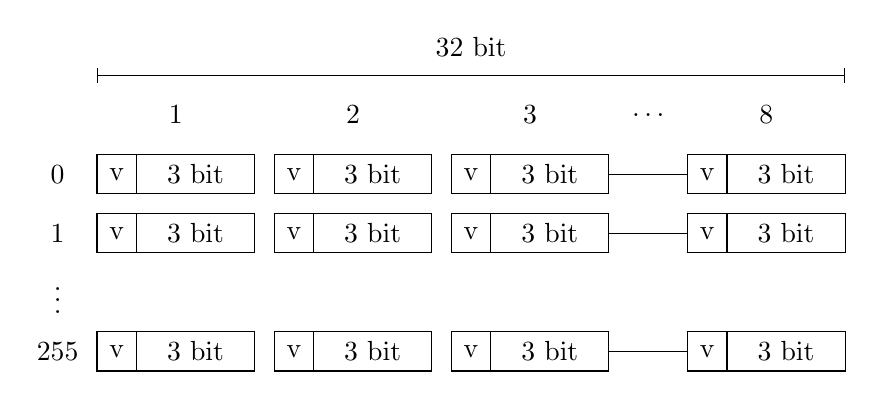
\begin{tikzpicture}
        \draw[|-|] (0,1.5) -- node[label=above:32 bit] {} ++(9.5,0);
        
        \foreach \x in {1,...,3} \draw (\x*2.25-1.25,1) node {\x};

        \draw (7,1) node {$\dots$} ++ (1.5,0) node {8};

        \foreach \x in {0,...,1,3}
        \draw (0,-\x*.75) rectangle node {v} ++(.5,.5) ++(0,-.5) rectangle node {3 bit} ++(1.5,.5)
            ++(.25,-.5) rectangle node {v} ++(.5,.5) ++(0,-.5) rectangle node {3 bit} ++(1.5,.5)
            ++(.25,-.5) rectangle node {v} ++(.5,.5) ++(0,-.5) rectangle node {3 bit} ++(1.5,.5)
            ++(0,-.25) -- node {} ++(1,0)
            ++(0,-.25) rectangle node {v} ++(.5,.5) ++(0,-.5) rectangle node {3 bit} ++(1.5,.5);

        % \draw (0,3) rectangle node {v} ++(.5,.5) ++(0,-.5) rectangle node {3 bit} ++(1.5,.5);

        \draw (-.5,.25) node {0} 
            ++(0,-.75) node {1}
            ++(0,-.75) node {$\vdots$}
            ++(0,-.75) node {255};

    \end{tikzpicture}
    \caption{Byte select lookup table}
    \label{fig:select_lookup}
\end{figure}

\section{Evaluation}
In this chapter we will evaluate our predicted runtime against measurements.
For the pre-computation we calculate an incremental sum $\prevsum$ every 7 blocks of 64 bits.
This should scale linearly with the vector size $|\vec{V}|=n$.
As for \code{rank} we can calculate the position of the vector line in constant time.
For \code{select} we need to first run a binary search in $\mathcal{O}(\log{n})$ to find the vector line.
After that we compute a linear search in $\mathcal{O}(7)$ as there is a maximum of 7 blocks we need to search.
The runtime should be dominated by the binary search.
To validate these predictions we conducted an experiment were a bitvector $\vec{V}$ with increasing
size was randomly generated as well as a fixed amount of $100 000$ commands.
We then measured the runtime for the pre-computation as well as the command execution.
In Figure~\ref{fig:performance_eval} the recorded data is visualized.
\begin{figure}[t]
    \centering
    \begin{tikzpicture}
    \begin{groupplot}[group style={group size= 2 by 1},height=6cm,width=.45\textwidth]
        \nextgroupplot[
            legend columns=-1,
            legend to name=usageLegend,
            ymin=1,
            ymax=1000,
            ymode=log,
            log basis y=10,
            ylabel={runtime},
            xlabel={vector size},
            y SI prefix=milli,
            y unit=s,
            xmin=27,
            xticklabel={$2^{\pgfmathparse{\tick}\pgfmathprintnumber{\pgfmathresult}}$},
            enlarge x limits=auto,
            grid=both,
            tick align=outside,
            tickpos=left,
            title=Intel,
        ]
        \addplot [
            mark=+,
            error bars/.cd,
                y dir=both,
                y explicit,
        ] table [x=bits,y=mean,y error=error] {benchmarks/framework.dat};
        \addlegendentry{Runtime}
                
        \addplot [
            mark=+,
            color=red,
            error bars/.cd,
                y dir=both,
                y explicit,
        ] table [x=bits,y=commandMean,y error=commandError] {benchmarks/framework.dat};
        \addlegendentry{Command Execution}

        \addplot [
            mark=+,
            color=blue,
            error bars/.cd,
                y dir=both,
                y explicit,
        ] table [x=bits,y=precomMean,y error=precomError] {benchmarks/framework.dat};
        \addlegendentry{Precomputation}

        \coordinate (topleft) at (rel axis cs:0,1);% coordinate at top of the first plot

        \nextgroupplot[
            ymode=log,
            ymin=1,
            ymax=1000,
            log basis y=10,
            xlabel={vector size},
            xmin=27,
            yticklabel=\empty,
            xticklabel={$2^{\pgfmathparse{\tick}\pgfmathprintnumber{\pgfmathresult}}$},
            enlarge x limits=auto,
            grid=both,
            tick align=outside,
            tickpos=left,
            title=AMD,
        ]

        \addplot [
                mark=+,
                color=black,
                error bars/.cd,
                    y dir=both,
                    y explicit,
            ] table [x=bits,y=mean,y error=error] {benchmarks/hetzner.dat};
                    
            \addplot [
                mark=+,
                color=red,
                error bars/.cd,
                    y dir=both,
                    y explicit,
            ] table [x=bits,y=commandMean,y error=commandError] {benchmarks/hetzner.dat};

            \addplot [
                mark=+,
                color=blue,
                error bars/.cd,
                    y dir=both,
                    y explicit,
            ] table [x=bits,y=precomMean,y error=precomError] {benchmarks/hetzner.dat};

        \coordinate (topright) at (rel axis cs:1,1);% coordinate at top of the second plot
        

    \end{groupplot}
    \path (topleft)--(topright) coordinate[midway] (group center);
    \node[align=center,above,yshift=.8cm] at(group center) {\pgfplotslegendfromname{usageLegend}};
\end{tikzpicture}
    \caption{%
        Performance Evaluation of an increasing vector size and a constant 100 000 commands.
        The benchmark was run on both:
        a 12th Gen Intel® Core™ i5-1240P × 16 with 32 GiB RAM, 1 TB SSD running Fedora Linux 40
        and on a dedicated vCPU Server (Hetzner CCX33) with 
        8 Cores, 32 GiB RAM and 240 GiB SSD running on AMD Milan EPYC™ 7003 running Ubuntu 24.04.
    }
    \label{fig:performance_eval}
\end{figure}
Analyzing our data we can confirm the predicted runtime, where the pre-computation scales linearly
with the vector length, and the command execution time scaling logarithmic.
We also notice that the pre-computation on the AMD setup being faster while the command execution being
slower in comparison to the Intel setup.

%%
%% Bibliography
%%

%% Please use bibtex, 

% \bibliography{lipics-v2021-sample-article}

\appendix

\section{Code}
The code for this implementation can be found on Github in the following repository: 
\url{https://github.com/paulheg/kit_advanced_data_structures}.



\end{document}
